\chapter{案例研究}
\label{ch5}
	温控系统是智能建筑的重要组成部分之一,在本章,我们以一个智能办公建筑为例,研究该智能建筑中温控系统的作用,以验证本文所提方法的可行性和实用性。案例改编自Ansgar等学者在\citep{DBLP:conf/hybrid/FehnkerI04} 中提出的Room Heating Benchmark,与之前的研究\citep{DBLP:journals/chinaf/DavidDLMS12,不确定环境下智能大厦空调系统调度策略评估,DBLP:conf/compsac/ChenGCDLS15}相比,本案例考虑了更多实际因素:物理环境温度变化的实际模型、办公场景下用户行为的各种模式、人的散热对室内温度的影响以及实时电价的差异。此外,在\citep{DBLP:journals/chinaf/DavidDLMS12,不确定环境下智能大厦空调系统调度策略评估,DBLP:conf/compsac/ChenGCDLS15}中,研究人员根据自己的专业知识,直接给出了系统的可验证模型。而本案例展示了利用领域本体指导构建系统初步模型、模型精化、借助模型转换技术得到系统的ESHA,实现有关系统能耗等性质的验证与分析的完整过程。
	
\section{场景描述}
	一个智能办公建筑中包含一定数目的办公室、会议室和加热器。加热器的数量比房间少,且每个房间最多只能使用一个加热器。由于墙的热传导性,不断变化的外界环境温度以及相邻房间温度会对某个房间的室内温度造成影响。同时,办公建筑中的用户行为也会间接影响室内温度。加热器由一个简单恒温器控制,当房间温度低于某个特定阈值时,加热器打开;当房间温度高于某个特定阈值时,加热器关闭。在智能温控系统中,能耗主要来源于加热器的工作以及系统中的信号传输。
	%由于墙的热传导性,不同房间之间以及房间与外界环境之间存在热传递。对于房间i,与其他房间的热交换系数记作$a_{i,j}$,	与物理环境的热交换系数记作$b_{i}$,加热器对其作用的功率记作$c_{i}$。
	
\section{系统建模}
\subsection{初步模型}	
	依照第三章给出的智能建筑领域本体,我们首先对系统进行需求分析,并指导建模系统的扩展MARTE/UML初步模型。	
	\begin{figure}[!t]
	\centering
	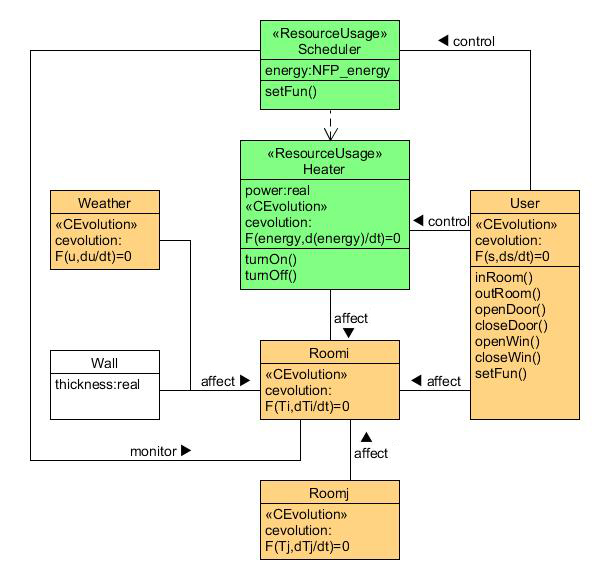
\includegraphics[width=3.8in]{sb-cd.jpg}
	\caption{智能办公建筑的类图}
	\label{sb-cd}
	\end{figure}
	
	\begin{figure}[!t]
	\centering
	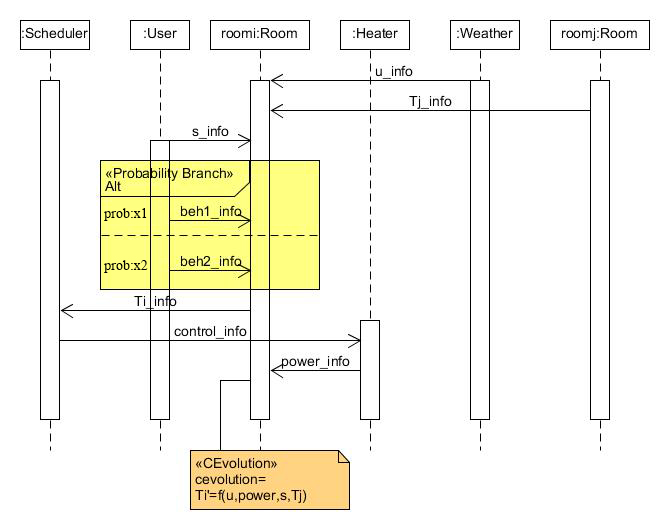
\includegraphics[width=4.2in]{sb-sd.jpg}
	\caption{智能办公建筑的顺序图}
	\label{sb-sd}
	\end{figure}
	
	\begin{figure}[!t]
	\centering
	\subfigure[物理环境]{
	\begin{minipage}[b]{0.3\textwidth}
	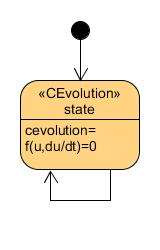
\includegraphics[width=0.6\textwidth]{weather-sm1.jpg} 
	\end{minipage}
	\label{weather-sm1}
	}
	\subfigure[加热器]{
	\begin{minipage}[b]{0.4\textwidth}
	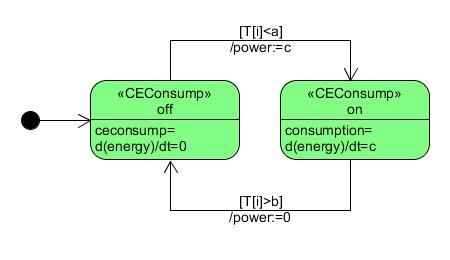
\includegraphics[width=1.2\textwidth]{heater-sm1.jpg} 
	\end{minipage}
	\label{heater-sm1}
	}
	\subfigure[室内环境]{
	\begin{minipage}[b]{0.3\textwidth}
	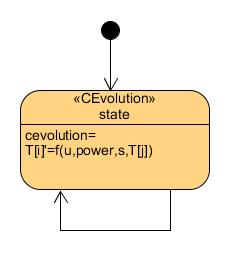
\includegraphics[width=0.8\textwidth]{room-sm1.jpg} 
	\end{minipage}
	\label{room-sm1}
	}
	\caption{物理环境、加热器和室内环境的初步状态图}
	\label{sm1}
	\end{figure}
	
	\begin{itemize}
	\item 首先,易知,在本案例中,我们研究的建筑环境参数是室内温度;
	\item 结合2.1.3节中定义的室内环境参数约束的第二条,可以找到相关的概念有:物理环境温度、相邻房间温度、墙的热传导性能、用户的离开/进入房间行为、开/关门行为、开/关窗行为、人的散热、加热器的作用以及调度器对加热器的控制;
	\item 根据概念间的相关关系,可以确定,涉及到的系统实体概念有:物理环境、加热器、房间室内环境、墙、用户和调度器,利用扩展的MARTE类图的定义,为它们分别创建如图\ref{sb-cd}所示的类图,前述的参数概念和行为概念对应各自类的属性和操作。易知,在智能温控系统中,耗能类是加热器和调度器,在之后的状态图建模中,我们将密切关注能量在对象内部的产生与消耗情况;
	\item 根据概念的上下文图(图\ref{context}),可知:物理环境和相邻房间的实时温度参数会影响室内环境;用户的散热和随机行为也会影响室内环境;加热器受调度器的控制,且其作用会对室内环境造成影响。而墙这种物理构成的参数是一个固定值,无需对其创建对象。基于上下文图,可建模如图\ref{sb-sd}所示的扩展MARTE/UML顺序图。首先,物理环境和相邻房间的温度信息会传递给当前房间$room_{i}$;用户自身的散热会影响室内温度,同时,用户有一定的概率执行随机行为$beh1$,一定的概率执行随机行为$beh2$,且其行为也会对室内温度造成影响;调度器以一定频率监测$room_{i}$的温度,并按照某种调度策略来控制加热器;加热器的加热功率直接影响室内温度;在$room_{i}$的控制焦点上,我们添加了$CEvolution$衍型来定义室内环境与其他因素的函数关系;
	\item 依照2.2节中给出的不同实体概念的模板构建状态图:对于物理环境,由于系统无法对其产生控制和影响,即它的状态不会被改变,因此,在状态图中,可以用表达式来描述物理环境参数的变化;对于加热器,在不考虑异常情况时,它通常应该在开启和关闭两个状态间切换,关闭时不耗能,开启时以一定速率耗能,且开启时其对室内环境的作用为其功率参数;对于用户,其行为是随机的,且每一个行为的发生会改变其状态;对于调度器,在一定的判断准则下,对加热器进行控制,且控制信号的传输会带来能耗;对于室内环境,它的温度参数受到以上几个实体的作用而变化。通过以上分析,可以得到物理环境、加热器和室内环境的初步状态图,如图\ref{sm1}所示。以上模型的状态变化符合一定的规则,可以抽象为固定模板,而用户行为具有较强的随机性,系统调度器的判断逻辑较为复杂,在下一节,我们将通过深入分析,给出办公场景下几种常见的用户行为模式和调度器的几种不同策略。
	\end{itemize}

\subsection{精化模型}
	在智能温控系统中,物理环境温度、室内温度和系统能耗的连续变化体现了系统的混成特性;而系统的随机性主要体现在用户行为的不确定;系统能耗的产生主要来源于两方面——加热器的工作、调度器和加热器之间的信号传输,其他对象通过影响调度器对加热器的决策间接影响能耗。	
	
	%在预设的场景中,由于加热器的数量少于房间数量,当出现多个房间需要加热器时,房间之间会产生竞争关系。此时,调度器必须按一定的规则对加热器进行调度。因此,对温控系统建模的一个重点是调度器的设计。通过领域本体可以指导我们建模智能建筑中的物理环境、室内环境和功能构件这些行为模式比较固定的实体概念的状态图。而对于系统调度器和用户这些实体,其内部状态变化较为复杂,下面,我们通过深入分析来进一步精化系统模型。
		
	在智能建筑领域本体中,我们已经定义了:室内温度与外界温度(物理环境温度和相邻空间温度)、墙的热传导性能、用户的离开/进入房间、开/关门行为、开/关窗行为、人的热量、暖通空调的作用以及调度器的控制有关。在本案例中,为了简化模型,对于用户行为仅考虑其离开/进入房间的影响。参考文献\citep{DBLP:conf/hybrid/FehnkerI04},本案例中房间i的室内环境温度可以由以下公式定义:
	
	\begin{equation}
	T_{i}^{'} = \sum_{j\not=i} a_{i,j}(T_{j}-T_{i})+b_{i}(u-T_{i})+c_{i}h_{i}+s(T_{i})N_{i}
	\label{gongshi}
	\end{equation}
	
	其中,变量$T_{i}$和$T_{j}$分别表示房间i和房间j的室内温度,变量$u$代表物理环境温度。$h_{i}$是一个布尔类型的变量,其值为1时代表加热器被房间i使用,其值为0时代表房间i并未使用加热器。常量$a_{i,j}$称作房间i和房间j的热交换系数,由墙的热传导性能和房间之间的相互位置决定。热传导系数具有对称性,即$a_{i,j}=a_{j,i}$,若房间i和房间j不相邻,则$a_{i,j}=0$。常量$b_{i}$和$c_{i}$分别表示房间i与物理环境的热传递系数和加热器对房间i的加热功率。$s(T_{i})$是指在室内温度为$T_{i}$的情况下人体产生的热量,$N_{i}$代表房间i内的人数。之前关于智能建筑温控系统的研究中均没有考虑到人的散热,实际上,在人数较多的办公环境中,对于室内温度而言,人的散热会带来不可忽略的影响。

	按照一个成年人的平均体重为68公斤的标准,结合\citep{CarrierCorporation1965Handbook}中人在不同温度下散热的数据,我们使用MATLAB工具进行仿真拟合,得到了人体散热与房间温度的关系为:
	\begin{equation}
	s(T)=98.62e^{-(\frac{T-14.03}{17.41})^2}
	\end{equation}
	%Each heater is equipped with a bang-bang controller congured to turn the heating on (hi := 1) when temperature Ti falls below the predened threshold oni and turn it back o (hi := 0) when temperature Ti becomes greater than oi . The central controller can switch over the heating from one room to another.290 Provided that there are two or more rooms that need to be heated at the same time, the controller may reallocate heaters according to predened strategies. By this way, heaters are shared by dierent rooms to meet some requirements on occupant comfortability or energy consumption. The room needs a heater if the temperature drops below its get threshold. The occupants feel uncomfortable when the room temperature drops below low. The controller adopts various control strategies to maintain the room temperature for 295 comfortable occupant feeling or optimize energy consumption. The denition and default setting of oni ,oi , get and low can be found in
	
	每个加热器由一个``bang-bang controller''控制:当房间i的温度$T_{i}$低于预设的开启温度$on_{i}$时,加热器开启,并将变量$h_{i}$置为1;当房间i的温度$T_{i}$高于预设的关闭温度$off_{i}$时,加热器关闭,并将变量$h_{i}$置为0。调度器可以将加热器从一个房间切换到另一个房间。当有超过两个房间同时需要加热时,调度器将使用某种策略来对加热器进行配置。通过这种方式,加热器得以被不同的房间共享使用,来保证室内用户的舒适度。当房间i的温度低于$get_{i}$($get_{i}<on_{i}$)时,代表它需要加热器。用户在房间的温度低于$low_{i}$($low_{i}<get_{i}$)时,会感到不舒服。调度器的智能控制需要保持室内温度在用户舒适度的范围内且尽量优化能耗。关于$on_{i}$、$off_{i}$、$get_{i}$和$low_{i}$的详细定义可以参考文献\citep{DBLP:conf/compsac/ChenGCDLS15}。
	
	在本案例中,我们考虑三种参数维度:
	\begin{enumerate}
	\item 物理环境温度:我们设计了四种不同的温度模拟方式,包括恒温、简单正弦函数模拟、复杂正弦函数模拟和高斯函数模拟;
	\item 调度策略:我们使用了三种调度策略,主要差异在于加热器使用权移动的判断方式不同;
	\item 用户行为模式:考虑到实际智能建筑中常见的办公情形,我们设计了三种用户行为模式,分别为日常工作模式、工作/出差模式和会议模式。在不同的用户行为模式中,用户行为通过改变上述的预设值——$on_{i}$、$off_{i}$、$get_{i}$和$low_{i}$和公式\ref{gongshi}中的系数,来影响调度器的调度,从而影响系统能耗。
	\end{enumerate}

\textbf{1、精化后的物理环境模型}

	\begin{figure}[!t]
	\centering
	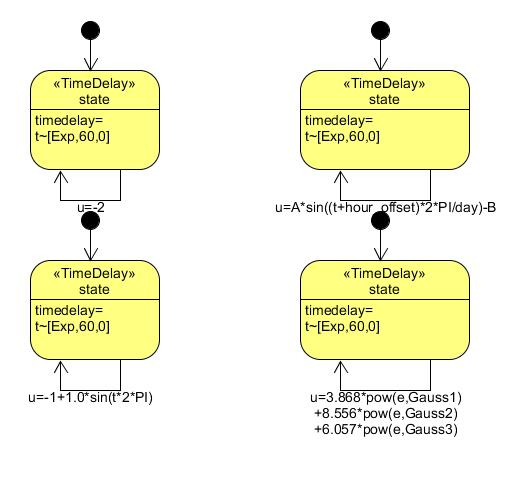
\includegraphics[width=3.2in]{weather-sm2.jpg}
	\caption{精化后的物理环境状态图}
	\label{weather-sm2}
	\end{figure}
	
	对于物理环境,不同于初步模型中直接将温度模拟公式附在状态上的方式。考虑到现实情况中,智能建筑的传感器按照一定频率对物理环境温度进行监测,我们将模型进行调整:将温度模拟公式添加到迁移上,并为状态设置一个指数型的时延概率分布,表示系统以每个时间单位60次的频率监测物理环境温度。
	
	如图\ref{weather-sm2}所示:图a表示物理环境恒定温度为-2摄氏度;图b表示一个简单的正弦函数模拟的温度;图c中的参数A和B为自定义值,可以更准确地模拟温度的实际情况;图d中的温度由高斯函数模拟,是我们根据上海2-3月份的实际温度情况在MATLAB工具中模拟后计算所得,最终的高斯曲线拟合结果为$u = 3.868e^{gauss1(t)} + 8.556e^{gauss2(t)} + 6.057e^{gauss3(t)}$,其中$gauss1(t) = -(\frac{t-23.16}{11.58})^2$,$gauss2(t) = - (\frac{t-14.24}{6.194})^2$,$gauss3(t) = -(\frac{t+1.212}{5.069})^2$。

\textbf{2、精化后的加热器模型}

	\begin{figure}[!t]
	\centering
	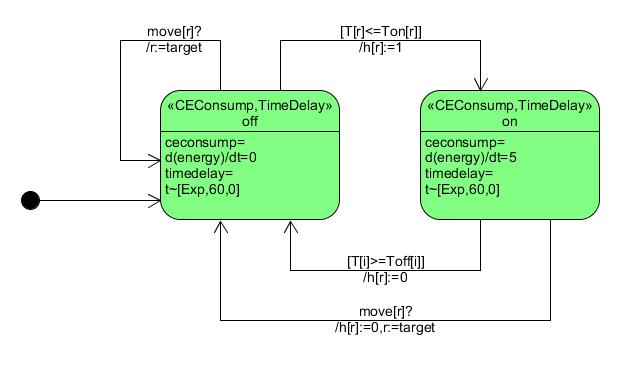
\includegraphics[width=3.8in]{heater-sm2.jpg}
	\caption{精化后的加热器状态图}
	\label{heater-sm2}
	\end{figure}
	
	在考虑了调度器的调度策略后,加热器在开启和关闭状态时必须接收来自调度器的信号,以确认是否转移作用的房间。当加热器关闭时,接收到调度器发送的$move[r]?$信号时,将变量$target$的值赋给$r$,即锁定将要判断的为房间r的温度;当加热器开启时,需要先将加热器使用权从当前的房间r夺走,再将$target$的值赋给$r$。此外,设置布尔型标记$h[i]$来表示房间i是否占有加热器,$h[i] \times c[i]$表示加热器对房间i的作用,则无需在开关状态切换时对加热功率$power$进行重新赋值。精化后的加热器状态图如图\ref{heater-sm2}所示。
	
\textbf{3、精化后的室内环境模型}

	\begin{figure}[!t]
	\centering
	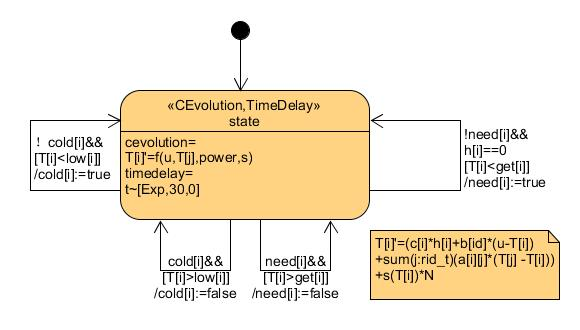
\includegraphics[width=3.6in]{room-sm2.jpg}
	\caption{精化后的室内环境状态图}
	\label{room-sm2}
	\end{figure}
	
	对于室内环境来说,结合前述关于$on_{i}$、$off_{i}$、$get_{i}$和$low_{i}$的介绍,我们将对室内温度的判断加在室内环境状态图中,并通过设置一些标记值来供调度器判断。如图\ref{room-sm2}所示,当房间i室内温度$T[i]$低于预设值$low[i]$时,代表室内温度已经不满足人的舒适度要求,将标记变量$cold[i]$置为$true$,反之为$false$;当$T[i]$高于预设值$get[i]$时,代表在当前的室内温度下,已经不需要加热器了,将标记变量$need[i]$置为$false$,反之为$true$。
	
\textbf{4、用户行为模型}
	\begin{figure}[!t]
	\centering
	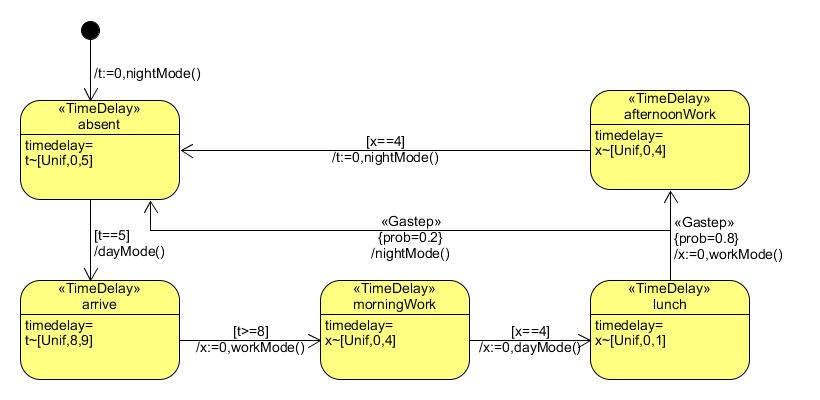
\includegraphics[width=4.8in]{user-sm.jpg}
	\caption{工作/出差模式状态图}
	\label{user-sm}
	\end{figure}
	
	在领域本体中,我们介绍了用户可以执行的行为,如离开/进入房间、开/关门、开/关窗等。之前的研究仅考虑了用户进入/离开房间这样的简单动作行为,本案例更贴合实际,考虑了办公场景中,职工的上班、下班、出差和开会这些常见的行为,并设计了三种用户行为模式:1)日常工作模式:用户早晨来到办公室上班、进行上午的工作、离开办公室去吃午饭、进行下午的工作,最后下班离开办公室;2)工作/出差模式:除了正常工作外,职工在下午可能会出差拜访客户等,由此可以设置工作/出差模式;3)会议模式:在某个项目刚开始的时期,为了确定项目方案,职工可能早上、下午均需要去会议室参加会议商讨方案。
	
	图\ref{user-sm}展示了工作/出差模式的状态图。最初,在凌晨至上午5点,办公建筑处于夜间模式,此时的$on_{i}$、$off_{i}$、$get_{i}$数值均处于预设的较低值;上午5点之后,办公建筑进入预热状态,即被$on_{i}$、$off_{i}$、$get_{i}$被设定为更高的值,开启白天模式;职工可能在上午8点至9点间的任意时刻来到办公建筑,当职工到达后,办公建筑被配置为工作模式,即对于室内环境来说,需要考虑办公室中人群的散热情况;之后,职工开始上午的工作,工作4小时后,他们会出去吃午饭,此时办公建筑再次被配置为白天模式,即不考虑人的散热情况;午饭时间为[0,1]时内的均匀分布,午饭回来后,职工有$80\%$的可能性继续下午的工作,$20\%$的可能性出去见客户,即直接离开办公建筑;若职工继续下午的工作,将连续工作4小时后下班,并离开办公建筑。
	
\textbf{5、调度器模型}	

	对于何时将房间j占有的加热器分配给房间i,即房间之间的竞争条件,我们考虑以下三种调度策略:	
	\begin{enumerate}
	\item 策略$\uppercase\expandafter{\romannumeral1}$:房间i的温度小于$get_{i}$,即$T_{i} < get_{i}$,且房间j和房间i的温差大于一定值,即$T_{j}-T_{i} \geq dif_{i}$;
	\item 策略$\uppercase\expandafter{\romannumeral2}$:房间i的温度小于$get_{i}$,即$T_{i} < get_{i}$,且房间j的温度大于$on_{j}$,即$T_{j} \geq on_{j}$;
	\item 策略$\uppercase\expandafter{\romannumeral3}$:房间i的温度小于$get_{i}$,即$T_{i} < get_{i}$,且房间j的温度大于$get_{j}$($get_{j}<on_{j}$),即$T_{j} \geq get_{j}$;
	\end{enumerate}

	下面,以策略$\uppercase\expandafter{\romannumeral1}$为例,我们将分析并给出调度器的扩展MARTE/UML状态图。
	
	\begin{figure}[!t]
	\centering
	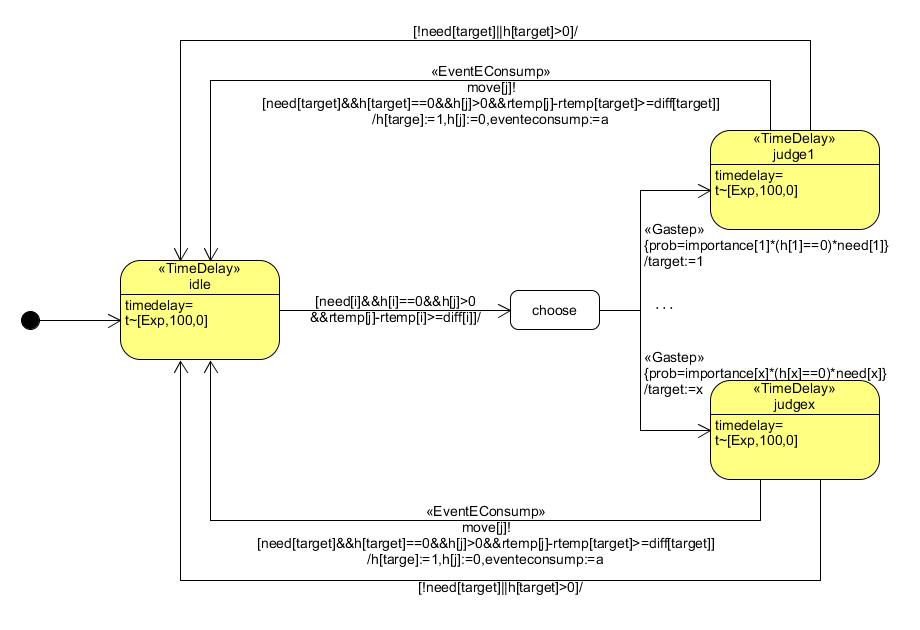
\includegraphics[width=4.9in]{scheduler-sm.jpg}
	\caption{策略$\uppercase\expandafter{\romannumeral1}$的状态图}
	\label{scheduler-sm}
	\end{figure}
	
	如图\ref{scheduler-sm}所示,当调度器处于空闲状态时,其以每单位时间(小时)100次的频率来监测室内环境的状态,这一随机行为由指数时延概率分布描述;当调度器监测到有房间需要加热且不占用加热器,同时存在另一个房间与其温差大于预设值$dif$时,调度器将发生状态迁移,进入选择状态;随后,调度器将对所有需要加热且不占用加热器的房间按照其重要性系数$imp$进行离散的概率选择;若调度器选择了房间x,则进入判断状态并将x设为加热器将要移动的目标$target$;随后,调度器判断此时是否仍存在一个占有加热器的房间,且其与房间x的温差大于$dif$,若成立,则将该房间的加热器赋予房间x,否则不执行任何操作。值得注意的是,在判断需要将某房间的加热器赋予房间x时,调度器会向该加热器发送信号,此时的信号传输需要消耗一定能量。
	
\section{模型验证与分析}
	在前面的系统建模步骤中,我们已经得到了系统的设计模型,但若要对系统进行验证,除了利用前述的转换算法将扩展的MARTE/UML状态图转换为ESHA模型外,还需要进行参数实例化,以验证特定参数组合下系统的性质,并分析系统的能耗。
	
	我们考虑一个具体的应用场景,某智能办公建筑的平面图如图\ref{building}所示,共包含一个会议室、五个办公室和三个加热器,且初始状态加热器1、加热器2、加热器3分别供房间2、房间4和房间6使用。
	
	\begin{figure}[!t]
	\centering
	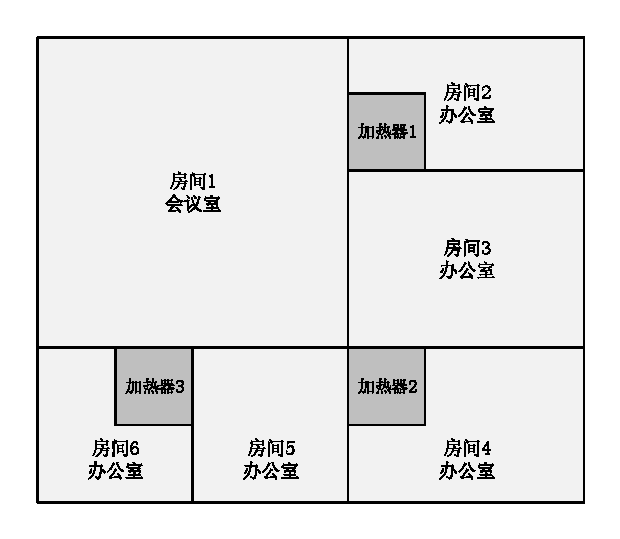
\includegraphics[width=3in]{building.pdf}
	\caption{智能办公建筑的布局}
	\label{building}
	\end{figure}
	
	在本案例中,参考文献\citep{DBLP:journals/chinaf/DavidDLMS12}中的数据,房间热交换系数、不同房间与物理环境的热交换系数和加热器对不同房间的加热功率设置如图\ref{room-para}。
	\begin{figure}
	\centering
	\subfigure[房间热交换系数]{
	\begin{minipage}[b]{0.3\textwidth}
	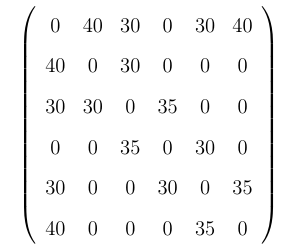
\includegraphics[width=1\textwidth]{aij.png} 
	\end{minipage}
	\label{aij}
	}
	\subfigure[物理环境热交换系数]{
	\begin{minipage}[b]{0.32\textwidth}
	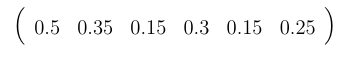
\includegraphics[width=1.1\textwidth]{bi.png} 
	\end{minipage}
	\label{bi}
	}
	\subfigure[加热器功率]{
	\begin{minipage}[b]{0.25\textwidth}
	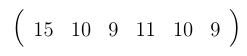
\includegraphics[width=1\textwidth]{ci.png} 
	\end{minipage}
	\label{ci}
	}
	\caption{案例参数实例化}
	\label{room-para}
	\end{figure}
%\begin{figure}
%\centering
%\subfigure[房间的热交换系数]{
%\begin{minipage}[b]{0.3\textwidth}
%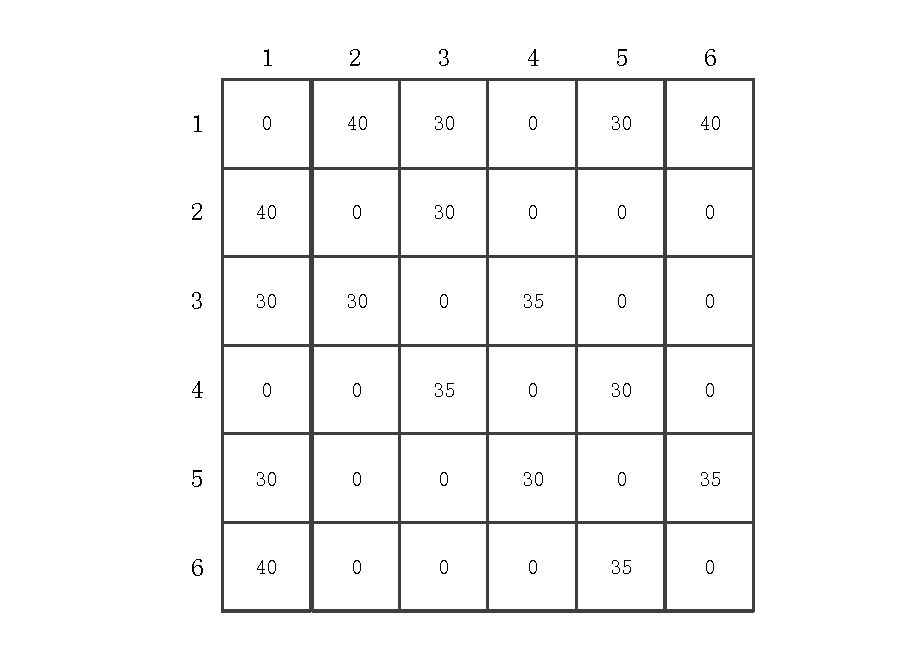
\includegraphics[width=1.5\textwidth]{room-a.pdf} 
%\end{minipage}
%\label{room-a}
%}

%\begin{equation}       
%\left(                 
%  \begin{array}{cccccc}   
%    0  & 40 & 30 & 0  & 30 & 40\\
%    40 & 0  & 30 & 0  & 0  & 0 \\
%    30 & 30 & 0  & 35 & 0  & 0 \\
%    0  & 0  & 35 & 0  & 30 & 0 \\
%    30 & 0  & 0  & 30 & 0  & 35\\
%    40 & 0  & 0  & 0  & 35 & 0 \\   
% \end{array}
%\right)                 
%\end{equation}

%\subfigure[不同房间与外界温度的热交换系数]{
%\begin{minipage}[b]{0.3\textwidth}
%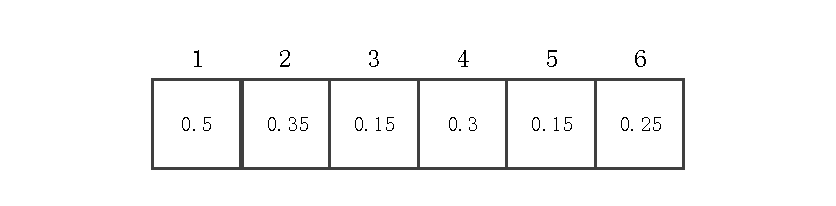
\includegraphics[width=1.5\textwidth]{room-b.pdf} 
%\end{minipage}
%\label{room-b}
%}
%\begin{equation}       
%\left(                 
%  \begin{array}{cccccc}   
%    0.5  & 0.35 & 0.15 & 0.3  & 0.15 & 0.25
%  \end{array}
%\right) 
%\end{equation}
%\subfigure[加热器对不同房间的功率]{
%\begin{minipage}[b]{0.3\textwidth}
%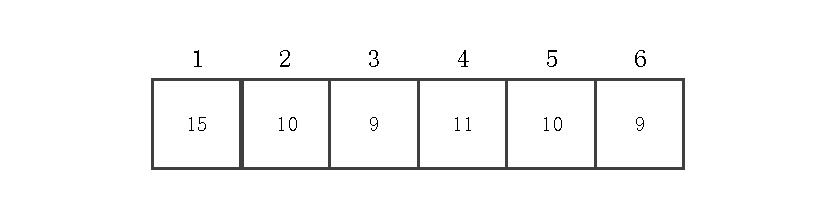
\includegraphics[width=1.5\textwidth]{room-c.pdf} 
%\end{minipage}
%\label{room-c}
%}
%\caption{案例参数实例化}
%\label{room-para}
%\end{figure}

%\begin{equation}     
%\left(                 
%  \begin{array}{c c c c c c c}   
%    15  & 10 & 9 & 11  & 10 & 9   
%  \end{array}
%\right)                 
%\end{equation}
\subsection{ESHA模型}
	对于本案例,完整的ESHA网络模型包括:物理环境模型、加热器模型、室内环境模型、用户行为模式模型、调度器模型和实时电价模型六部分。

	利用Modana模型转换器,我们将前述的MARTE/UML模型转换为UPPAAL工具可识别的ESHA模型,并使用UPPAAL工具载入该模型文件以图形化显示,为了模型的美观性,我们手动对模型进行了适当的修改(主要是将一些计算公式进行了函数封装)。
	
	图\ref{weather-esha}为四种物理环境模式的ESHA模型。其中,weatherGauss模型在$update()$函数中定义了如何利用高斯函数来模拟温度的具体公式。
	
	\begin{figure}
	\centering
	\subfigure[weatherFlat]{
	\begin{minipage}[b]{0.4\textwidth}
	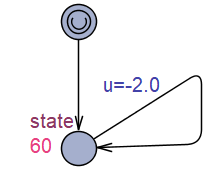
\includegraphics[width=0.45\textwidth]{weather-esha1.png} 
	\end{minipage}
	\label{weather1}
	}
	\subfigure[weatherSimple]{
	\begin{minipage}[b]{0.4\textwidth}
	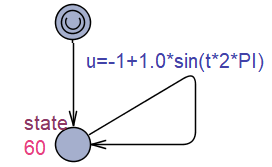
\includegraphics[width=0.6\textwidth]{weather-esha2.png} 
	\end{minipage}
	\label{weather2}
	}
	\subfigure[weatherComplex]{
	\begin{minipage}[b]{0.4\textwidth}
	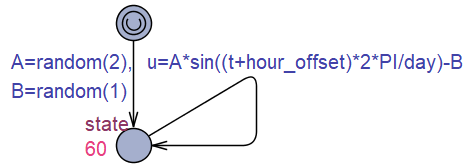
\includegraphics[width=1.0\textwidth]{weather-esha3.png} 
	\end{minipage}
	\label{weather3}
	}
	\subfigure[weatherGauss]{
	\begin{minipage}[b]{0.4\textwidth}
	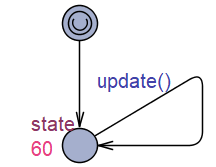
\includegraphics[width=0.45\textwidth]{weather-esha4.png} 
	\end{minipage}
	\label{weather4}
	}
	\caption{四种物理环境模式的ESHA模型}
	\label{weather-esha}
	\end{figure}
	
	图\ref{heater-esha}为加热器和室内环境的ESHA模型。
	
	\begin{figure}
	\centering
	\subfigure[heater]{
	\begin{minipage}[b]{0.4\textwidth}
	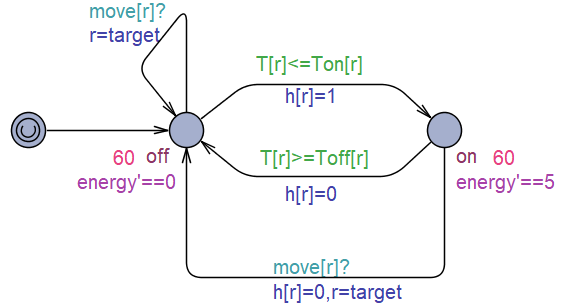
\includegraphics[width=1.05\textwidth]{heater-esha.png} 
	\end{minipage}
	\label{heater-esha}
	}
	\subfigure[room]{
	\begin{minipage}[b]{0.4\textwidth}
	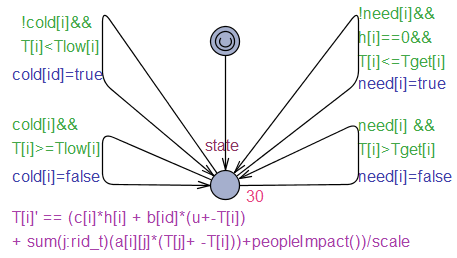
\includegraphics[width=1.05\textwidth]{room-esha.png} 
	\end{minipage}
	\label{room-esha}
	}
	\caption{加热器和室内环境的ESHA模型}
	\label{heater-esha}
	\end{figure}

	如前文所述,用户模式分为日常工作模式、工作/出差模式和会议模式,三种用户模式的ESHA模型如图\ref{user-esha}所示。
	
	\begin{figure}
	\centering
	\subfigure[work]{
	\begin{minipage}[b]{0.4\textwidth}
	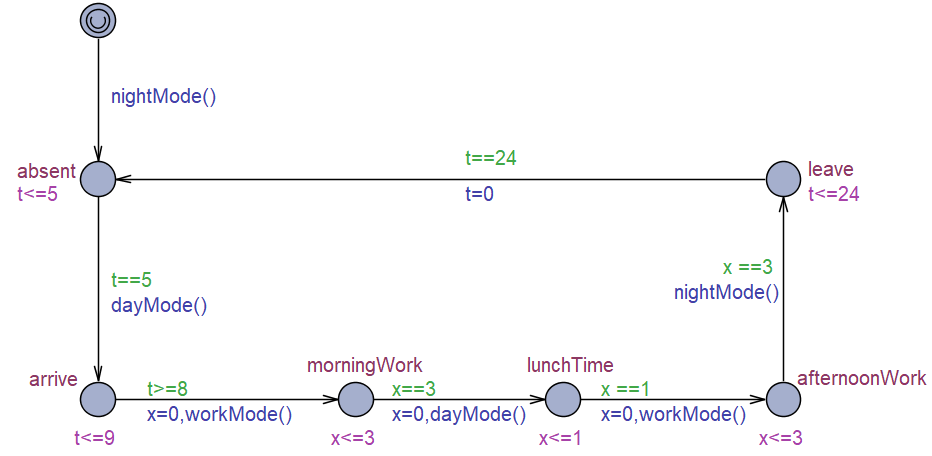
\includegraphics[width=1.05\textwidth]{user-esha1.png} 
	\end{minipage}
	\label{user-work}
	}
	\subfigure[work/out]{
	\begin{minipage}[b]{0.4\textwidth}
	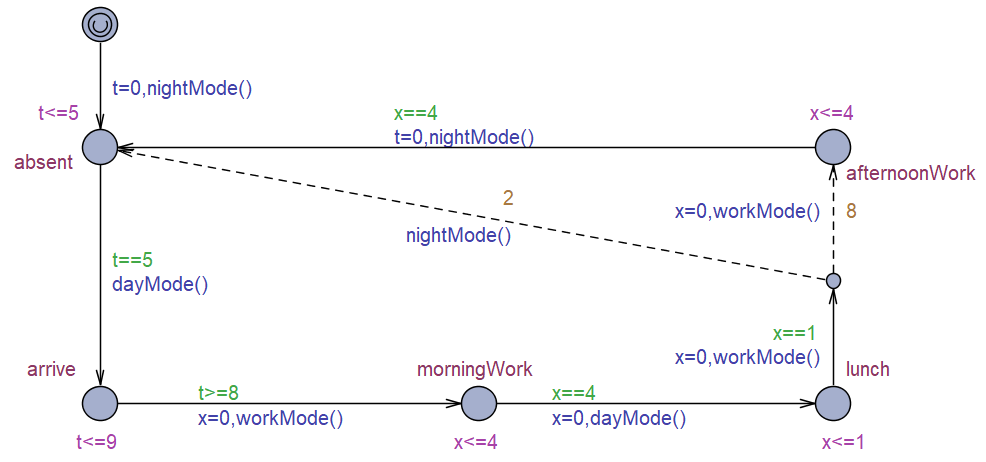
\includegraphics[width=1.05\textwidth]{user-esha2.png} 
	\end{minipage}
	\label{user-prob}
	}
	\subfigure[conference]{
	\begin{minipage}[b]{0.4\textwidth}
	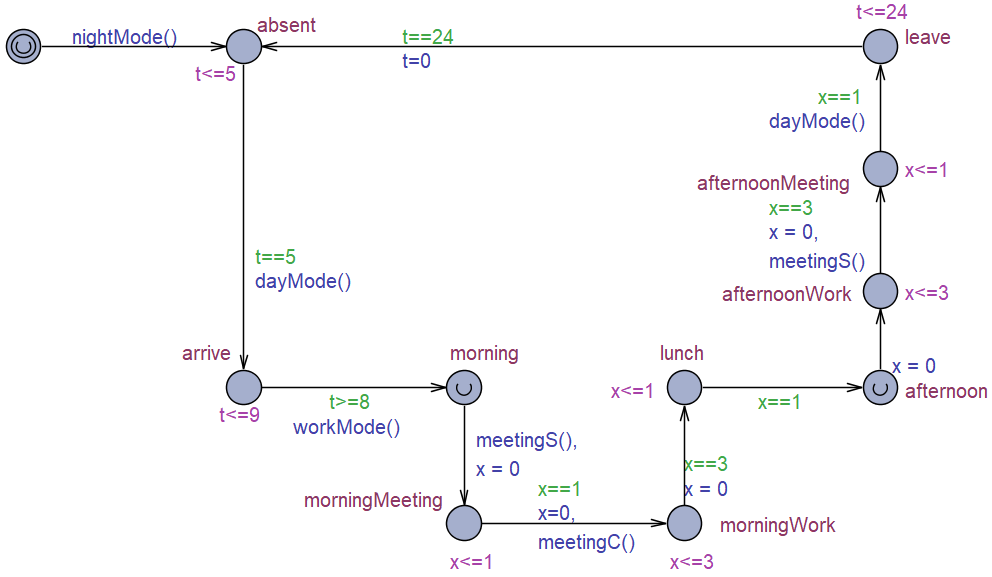
\includegraphics[width=1.05\textwidth]{user-esha3.png} 
	\end{minipage}
	\label{user-conference}
	}
	\caption{三种用户行为模式ESHA模型}
	\label{user-esha}
	\end{figure}
	
	在上一节,我们已经介绍了调度器的三种策略,并给出了策略$\uppercase\expandafter{\romannumeral1}$的状态图,图\ref{scheduler-esha}为三种策略的ESHA模型。

	\begin{figure}
	\centering
	\subfigure[strategy1]{
	\begin{minipage}[b]{0.4\textwidth}
	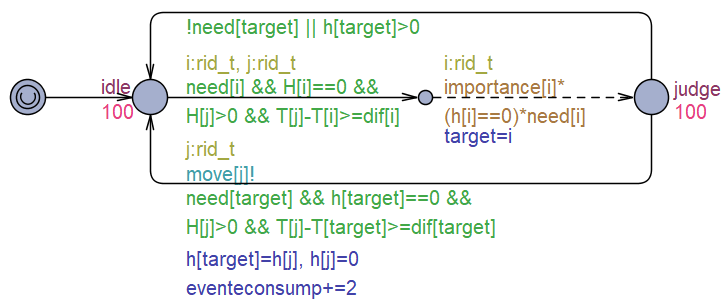
\includegraphics[width=1.05\textwidth]{scheduler-esha1.png} 
	\end{minipage}
	\label{scheduler1-esha}
	}
	\subfigure[strategy2]{
	\begin{minipage}[b]{0.4\textwidth}
	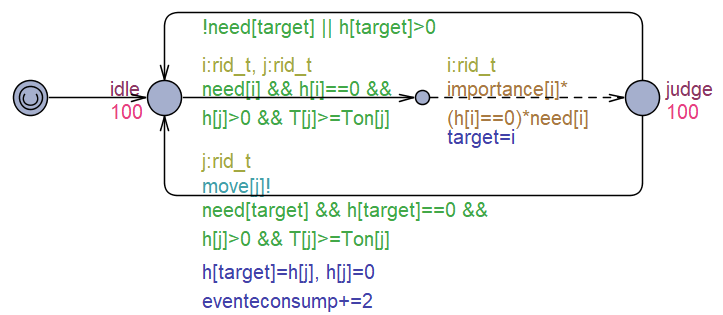
\includegraphics[width=1.05\textwidth]{scheduler-esha2.png} 
	\end{minipage}
	\label{scheduler2-esha}
	}
	\subfigure[strategy3]{
	\begin{minipage}[b]{0.4\textwidth}
	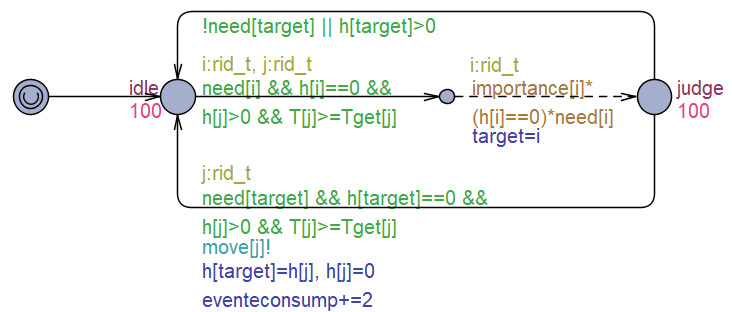
\includegraphics[width=1.05\textwidth]{scheduler-esha3.png} 
	\end{minipage}
	\label{scheduler3-esha}
	}
	\caption{三种策略的ESHA模型}
	\label{scheduler-esha}
	\end{figure}
	
	在现实生活中,为了鼓励人们错开用电高峰期,不同时段的电价是不相同的,对此,参考\citep{刘经浩2015一种基于实时电价的}我们构建了如图\ref{price}所示的实时电价ESHA模型。对于办公建筑,10点至14点是用电高峰期,此时的电价高于其他时间。
	
	\begin{figure}[!t]
	\centering
	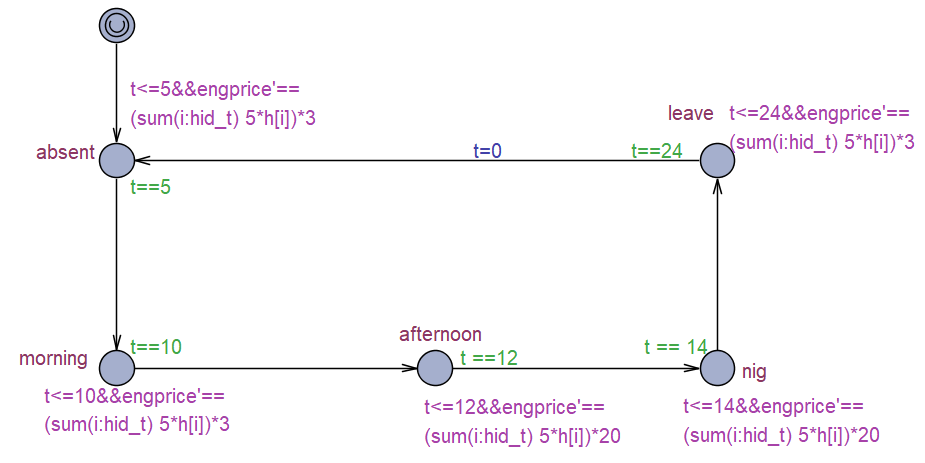
\includegraphics[width=3.8in]{price.png}
	\caption{实时电价的ESHA模型}
	\label{price}
	\end{figure}
	
\subsection{模型验证与分析}
\textbf{1、模型仿真}

	由于在本案例中,共有4种不同的物理环境模型、3种不同的调度策略和3种不同的用户行为模式,因此共有$4\times3\times3$种组合情况。首先,我们采用固定配置$(weatherGauss,strategy1,work/out)$对模型进行仿真,来探究系统的能耗等性质。图\ref{T}为某次仿真48小时内六个房间室内环境温度变化情况。从图中可以看出在8(32)到14(38)时之间,各房间的温度均维持在16度以上,这说明调度器的智能控制起了作用,使得不会有房间的温度过低。在38到42时房间的温度有所下降,是由于用户出差离开了办公室,导致办公建筑开启夜间模式所致。图\ref{energy-discomfort}为10次仿真下48小时内能耗和用户不舒适度情况。受到外界环境的影响,在0到12时和24到36时,由于物理环境温度过低,需要加热器大量耗能来对办公建筑进行加热,因此在这两个阶段,能量消耗较快。而用户的不舒适度同样也是在上述两个夜间阶段增幅较大,其余时间较为稳定,说明调度器的调度有效,在白天办公场景中,为用户提供了一个较舒适的环境。
	
	\begin{figure}
	\centering
	\subfigure[48小时内各房间的温度]{
	\begin{minipage}[b]{0.4\textwidth}
	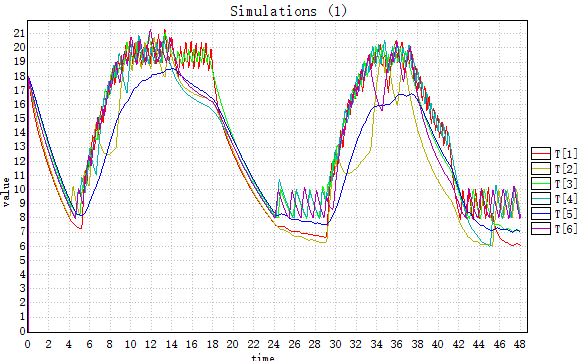
\includegraphics[width=1\textwidth]{T.png} 
	\end{minipage}
	\label{T}
	}
	\subfigure[48小时内系统能耗和用户不舒适度]{
	\begin{minipage}[b]{0.4\textwidth}
	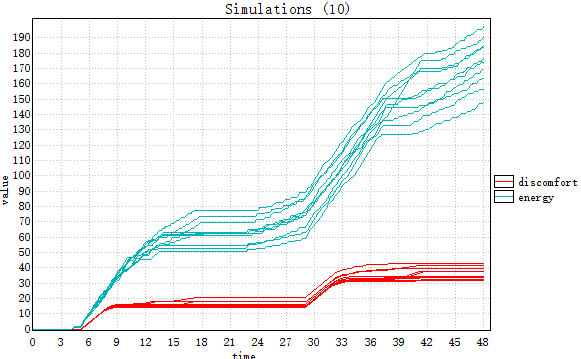
\includegraphics[width=1\textwidth]{energy-discomfort.png} 
	\end{minipage}
	\label{energy-discomfort}
	}
	\caption{系统仿真结果}
	\label{simulation}
	\end{figure}

\textbf{2、模型验证与分析}

	在以下情形中,我们将物理环境固定为weatherGauss模式,以探究不同调度策略和用户模式对系统能耗、用户不舒适度和电费的影响。
	
	\textbf{不同策略}:	
	
	为了验证不同策略对系统变量的影响,我们固定用户行为模式为工作/出差模式。
	图\ref{3strategy}所示为调度器的三种不同策略下,用户不舒适度、系统能耗和电费的概率密度图。由图(a)可知,在48小时内关于用户不舒适度的平均值,$strategy2<strategy3<strategy1$,即策略$\uppercase\expandafter{\romannumeral2}$能为用户提供一个更为适宜的温度环境;由图(b)可知,在48小时内关于系统能耗的平均值,$strategy2<strategy3<strategy1$,即策略$\uppercase\expandafter{\romannumeral2}$更加节能;由图(c)可知,在48小时内关于电费的平均值,$strategy1<strategy2<strategy3$,即策略$\uppercase\expandafter{\romannumeral1}$能够使得电费总额最小,但是三种策略的差异并不明显;综合以上三点考虑可知,策略$\uppercase\expandafter{\romannumeral2}$在能够在使得系统能耗和电费较少的情况下,提供更好的用户舒适度,其性能最优。
	
	\begin{figure}
	\centering
	\subfigure[用户不舒适度]{
	\begin{minipage}[b]{0.4\textwidth}
	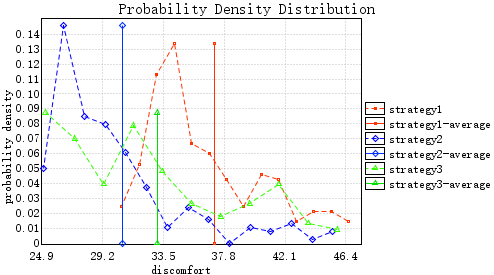
\includegraphics[width=1\textwidth]{s-dis.png} 
	\end{minipage}
	\label{dis-strategy}
	}
	\subfigure[系统能耗]{
	\begin{minipage}[b]{0.4\textwidth}
	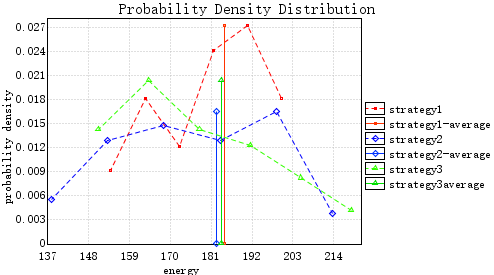
\includegraphics[width=1\textwidth]{s-energy.png} 
	\end{minipage}
	\label{energy-strategy}
	}
	\subfigure[电费]{
	\begin{minipage}[b]{0.4\textwidth}
	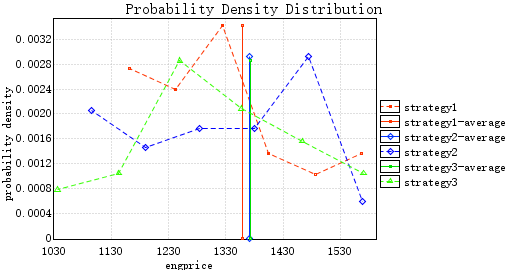
\includegraphics[width=1\textwidth]{s-price.png} 
	\end{minipage}
	\label{price-strategy}
	}
	\caption{三种策略对用户不舒适度、系统能耗、电费的影响}
	\label{3strategy}
	\end{figure}
	
	\textbf{不同用户行为模式}:
	
	为了分析不同的用户行为模式对系统变量的影响,我们将调度器策略固定为strategy1,在此配置下验证了三种用户行为模式对用户不舒适度、系统能耗和电费的影响,实验结果如图\ref{3user}所示。由图(a)可知,会议模式的用户不舒适度均值最低,工作/出差模式下的用户不舒适度均值最高,这是由于会议室的权重最高,调度器会优先维持会议室的温度,而工作/出差模式下用户的随机行为给调度器的智能控制带来了障碍;由图(b)可知系统能耗与用户的工作时间密切相关。在会议模式下,用户的工作时间为8小时,日常工作模式下用户的工作时间为6小时。对于工作/出差模式,用户的工作时间为$4+4 \times 0.8=7.2$小时。图(b)所示与上述分析一致,会议模式下系统能耗最高,日常工作模式下系统能耗最低;由图(c)可知,关于电费总额,工作/出差模式<日常工作模式<会议模式,这是由于电费与能耗值密切相关,会议室的能耗速率最高,且下午召开会议时,实时电价最高。
	
	\begin{figure}
	\centering
	\subfigure[用户不舒适度]{
	\begin{minipage}[b]{0.4\textwidth}
	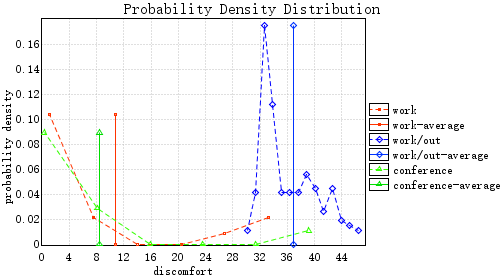
\includegraphics[width=1\textwidth]{u-dis.png} 
	\end{minipage}
	\label{dis-strategy}
	}
	\subfigure[系统能耗]{
	\begin{minipage}[b]{0.4\textwidth}
	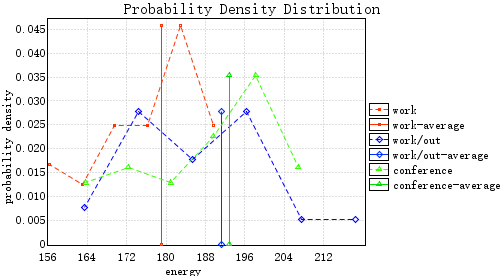
\includegraphics[width=1\textwidth]{u-energy.png} 
	\end{minipage}
	\label{energy-strategy}
	}
	\subfigure[电费]{
	\begin{minipage}[b]{0.4\textwidth}
	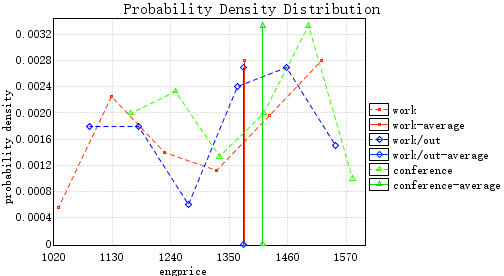
\includegraphics[width=1\textwidth]{u-price.png} 
	\end{minipage}
	\label{price-strategy}
	}
	\caption{三种用户行为模式对用户不舒适度、系统能耗、电费的影响}
	\label{3user}
	\end{figure}
	

\section{本章小结}
	智能建筑中的一个典型实例是智能温控系统,本章基于一个温控系统的benchmark,设计了一个更符合实际情境的实验案例,并将本文提出的智能建筑的能耗建模与分析方法进行了应用:从系统的需求出发,利用领域本体辅助构建扩展的MARTE/UML模型,模型转换为ESHA,最终利用UPPAAL-SMC工具实现了系统能耗等性质的验证与分析,探究了不同的调度策略和用户随机行为对系统能耗的影响。

	
	
	